\documentclass[conference]{IEEEtran}

\usepackage{booktabs}
\usepackage{amsmath}
\usepackage{amssymb}
\usepackage{tikz}
\usepackage{pgfplots}
\usetikzlibrary{arrows.meta,positioning,shapes.geometric}
\pgfplotsset{compat=1.18}

\title{Educational Multi-Agent Benchmarking: IEEE SMC 2026 Results Snapshot and Methodology}
\author{Anonymous Authors}

\begin{document}
\maketitle

\begin{abstract}
This section package reports a frozen snapshot of EduBench and TutorEval results for four architecture families (classical RAG, hybrid fast, non-RAG multi-agent, and single-agent no-RAG), interprets each metric under dataset-specific supervision semantics, and proposes a calibrated budget-aware successor architecture grounded in the present implementation.
\end{abstract}

% IEEE SMC 2026 style narrative section
% Grounded in src/eduagentic implementation and frozen snapshot artifacts.

\section{Result Snapshot, Metric Semantics, and Architecture Methodology}

\subsection{Snapshot Protocol and Scope}
All numbers in this package come from \texttt{frozen\_metrics\_snapshot.jsonl} in \texttt{latex\_tables\_metrics\_}, frozen at 2026-04-12 21:18:44 EDT from experiment result files under \texttt{artifacts/experiments/results/}. The most important protocol detail is that EduBench is still running while TutorEval is complete. At freeze time, EduBench coverage ranges from 4.02\% (classical RAG) to 13.31\% (hybrid fast), while TutorEval is 100\% complete for all four families (Table~\ref{tab:run_completion_snapshot}). We therefore read EduBench as a partial trajectory and TutorEval as a converged endpoint.

\subsection{How Metrics Are Computed in This Codebase}
The evaluator computes per-example metrics in \texttt{src/eduagentic/evaluation/metrics.py} and stores run summaries through \texttt{scripts/run\_eval\_session.py}. Summary fields are arithmetic means over successful records, and the output writer additionally records completion state (processed, pending, failed, resumed).

The lexical overlap core is standard. Exact Match is normalized string identity, and Token-F1 follows
\begin{equation}
F_1 = \frac{2PR}{P+R},\quad
P = \frac{|T_{pred} \cap T_{gold}|}{|T_{pred}|},\quad
R = \frac{|T_{pred} \cap T_{gold}|}{|T_{gold}|}.
\end{equation}

Grounding and educational supervision are profile dependent. Rubric coverage marks a rubric item as covered when either a lexical prefix appears or token overlap with that item exceeds 0.35. EduBench adds JSON compliance and score calibration:
\begin{equation}
\text{EduJSON} = \frac{\mathbb{1}(\text{score}) + \mathbb{1}(\text{scoring details}) + \mathbb{1}(\text{feedback})}{3},
\end{equation}
\begin{equation}
\text{EduAlign} = \max\left(0, 1 - \frac{|\hat{s} - s^*|}{100}\right).
\end{equation}
TutorEval instead activates keypoint precision/recall and chapter-grounding checks. Because profile gating is explicit in code, cross-profile metrics are intentionally left at 0.0 rather than estimated post hoc.

Efficiency fields are produced in \texttt{src/eduagentic/orchestration/pipelines.py}. Complexity units are explicitly defined as
\begin{equation}
\begin{aligned}
\text{ComplexityUnits} =\;& \text{TotalTokens} + 160\,\text{RetrievalQueries} \\
&+ 90\,\text{RetrievedChunks} + 240\,\text{AgentCount} \\
&+ 30\,\text{TraceEvents}.
\end{aligned}
\end{equation}
Reported complexity-per-second is computed per example and then averaged, which can diverge from a ratio computed from summary means.

\subsection{EduBench: Exhaustive Metric Reading at Current Freeze}
EduBench is a consensus-style supervision profile in which direct gold answers are typically unavailable in public rows. As a consequence, Exact Match, Token-F1, and choice accuracy are all 0.0 for every architecture in Table~\ref{tab:edubench_metric_inventory}. This is structural, not a behavioral collapse. In the same table, supervision\_available is 1.0 because rubric and reference-score style supervision are present through the adapter pipeline.

Grounding-linked fields split the methods into two clear regimes. Grounded overlap is 0.3384 for classical RAG and 0.0 for the other families. Citation coverage is 1.0 across all families, but this should not be read as universal citation quality: when no chunks are retrieved, the implementation returns a perfect coverage fallback. Retrieval doc recall is 0.0 throughout because expected document IDs are generally absent in this profile.

Rubric behavior strongly favors orchestrated variants in this partial run. Hybrid fast and non-RAG multi-agent reach 0.9553 and 0.9541 rubric coverage, well above classical (0.7987) and single-agent (0.7345). Adaptivity is 0.0 for all families, reflecting sparse dialogue-history triggers in this slice rather than inability to adapt.

The two EduBench-specific targets reveal a calibration-versus-structure trade-off. Edu JSON compliance remains low for all methods, with single-agent highest at 0.0209 and the other families between 0.0034 and 0.0049. Edu score alignment, however, is highest for classical RAG (0.2419), then single-agent (0.0933), non-RAG (0.0347), and hybrid (0.0302). The code-consistent interpretation is that retrieval anchoring helps score calibration, while specialist orchestration currently helps rubric language coverage more than strict score agreement.

The runtime layer shows equally strong trade-offs. Hybrid fast is currently the most efficient EduBench configuration in latency and tokens (29950.7 ms, 1757.8 tokens), while classical is much heavier (48170.2 ms, 3871.4 tokens). Relative to classical, hybrid reduces latency by 37.8\% and token use by 54.6\% while increasing rubric coverage by 19.6\%; the cost is an 87.5\% drop in score-alignment at this partial stage. Completion throughput also favors hybrid: 13.31\% processed versus 4.02\% for classical, a $3.31\times$ coverage multiple. Failure behavior remains most adverse in single-agent in normalized terms (6 failed out of 1344 processed).

\subsection{TutorEval: Exhaustive Converged Reading}
TutorEval is fully processed and therefore suitable for endpoint comparisons. Table~\ref{tab:tutoreval_metric_inventory} shows that exact match and choice accuracy remain 0.0 for all methods, while token-level overlap differentiates configurations. Hybrid fast reaches the best Token-F1 at 0.1152, followed by classical at 0.1115, then non-RAG (0.0898) and single-agent (0.0865).

Grounding and rubric fields reinforce this ordering for retrieval-aware quality. Hybrid has the best grounded overlap (0.2953) and rubric coverage (0.9902), with classical close behind (0.2812 and 0.9773). Non-RAG and single-agent have grounded overlap 0.0 by definition in this setting, but still retain high rubric coverage because rubric overlap is not retrieval-gated.

TutorEval-specific pedagogical metrics provide finer structure. Hybrid has the highest keypoint recall (0.8974), classical is second (0.8901), and non-RAG/single-agent trail at 0.8672 and 0.8423. Keypoint precision is nearly tied between classical (0.1134) and hybrid (0.1128), with the latter lower by only 0.0006 absolute. Chapter grounding is highest for non-RAG and single-agent (0.1445 and 0.1411), which is consistent with the implementation allowing chapter-context overlap fallback when retrieval chunks are absent.

Several metrics are effectively constants and should not be over-interpreted as discriminators here: citation coverage is 1.0 throughout due fallback behavior, retrieval doc recall is 0.0 because expected doc IDs are usually unavailable, adaptivity is 0.0 because dialogue-history cues are sparse, supervision availability is 1.0, and EduBench-specific metrics are profile-gated to 0.0.

On efficiency, hybrid is the strongest converged point in both wall-clock and token load (49113.4 ms and 3490.3 tokens), improving over classical by 5.37\% in latency and 12.19\% in tokens while also improving Token-F1, grounded overlap, rubric coverage, and keypoint recall.

\subsection{Cross-Dataset Architectural Interpretation}
The observed geometry is coherent with the implementation. Routing is provided by a lightweight regime router with dataset priors and heuristic evidence/coordination scores, and hybrid fast executes planner, diagnoser, and rubric specialists in parallel before conditional retrieval. This design explains why hybrid can remain cheaper than classical RAG even with more specialist roles: retrieval is invoked adaptively rather than unconditionally.

The retrieval subsystem is intentionally lightweight (TF-IDF variants, linear projection, reranking, MMR packing), which keeps specialist orchestration from automatically becoming latency-prohibitive. At the same time, current summaries expose two known caveats that matter for SMC reporting quality. First, API-time aggregates can exceed wall-clock latency because parallel branch latencies are summed. Second, profile-gated metrics produce legitimate structural zeros that should not be mixed into cross-profile claims.

\section{Proposed Novel Architecture: CBRH-2 (Calibrated Budgeted Reflective Hybrid)}

\subsection{Methodological Philosophy}
The next architecture should not simply add more specialist calls. The stronger principle is selective computation: spend additional budget only when uncertainty, pedagogical risk, and grounding risk jointly justify escalation. CBRH-2 therefore keeps the fast specialist backbone from hybrid fast, but turns escalation into an explicit constrained decision process with calibrated uncertainty and hard budget accounting.

\subsection{Decision Objective}
For each example, let $a$ denote an action from the set \{keep-fast-path, retrieve, critic-revise, architecture-escalate\}. We define expected utility as
\begin{equation}
\begin{aligned}
\mathbb{E}[U(a)] ={}& w_q\,\Delta Q(a) + w_g\,\Delta G(a) + w_p\,\Delta P(a) \\
&- \lambda_t\,\Delta T(a) - \lambda_k\,\Delta K(a) - \lambda_r\,\Delta R(a),
\end{aligned}
\end{equation}
where $\Delta Q,\Delta G,\Delta P$ are expected gains in quality, grounding, and pedagogy, and $\Delta T,\Delta K,\Delta R$ are expected latency, token, and retrieval-query costs. Escalation is allowed only when
\begin{equation}
\mathbb{E}[U(a)] > 0
\quad\text{and}\quad
(T,K,R) \preceq (B_T,B_K,B_R),
\end{equation}
with $(B_T,B_K,B_R)$ the remaining per-example budget.

\subsection{Controller Design}
CBRH-2 builds an uncertainty scalar
\begin{equation}
u = \alpha_1\,m_{router} + \alpha_2\,s_{critic} + \alpha_3\,d_{ground} + \alpha_4\,d_{pedagogy},
\end{equation}
where $m_{router}$ is routing margin uncertainty, $s_{critic}$ is issue severity, $d_{ground}$ is grounding deficit proxy, and $d_{pedagogy}$ is rubric/keypoint deficit proxy. The controller in Figure~\ref{fig:cbrh2_controller} escalates only when $u>\tau$ and the constrained utility test remains positive. This gives a principled way to preserve hybrid-like speed while recovering classical-like calibration when needed.

\subsection{Repository-Consistent Realization Path}
CBRH-2 is directly realizable in this repository without replacing the stack. The router already emits score vectors and can expose calibrated confidence margins. The critic can be upgraded from free-form issues to structured severity vectors. The pipeline finalizer already computes latency/tokens/retrieval counts and complexity units, providing immediate reward features for policy optimization. Finally, profile-aware adapters already separate EduBench and TutorEval supervision signals, enabling multi-objective training without forcing a single universal target.

\subsection{Research Methodology for SMC 2026}
The recommended study design is an offline-to-online sequence. First, fit calibration models and utility predictors from existing logs using doubly robust off-policy evaluation. Second, run constrained online experiments where escalation thresholds are swept under fixed budgets. Third, report Pareto fronts over educational quality, grounding quality, and compute cost, with profile-specific endpoints (EduBench: score calibration and JSON structure; TutorEval: keypoint recall and chapter grounding). This methodology transforms the benchmark from static comparison into adaptive decision-making research under realistic inference budgets.

\section{Validity and Reporting Constraints}
To remain publication-safe, all claims should preserve four constraints. EduBench remains partial at freeze time and should be reported as trajectory evidence, not final ranking. Cross-profile zeros are structural and should be interpreted as non-applicable rather than poor performance. Citation coverage and retrieval recall should be framed with fallback behavior caveats. Reported complexity-per-second should be accompanied by recomputed summary-ratio values (Table~\ref{tab:efficiency_decomposition}) to avoid over-reading mean-of-ratios artifacts.

% IEEE SMC 2026 style result tables
% Snapshot source: latex_tables_metrics_/frozen_metrics_snapshot.jsonl
% Snapshot timestamp: 2026-04-12 21:18:44 EDT

\begin{table*}[t]
\caption{Run-completion status at freeze time. EduBench sessions are still active; TutorEval sessions are converged.}
\label{tab:run_completion_snapshot}
\centering
\footnotesize
\begin{tabular}{llrrrrrr}
\toprule
Dataset & Architecture & Success & Processed & Total & Coverage (\%) & Pending & Failed \\
\midrule
EduBench & classical\_rag & 682 & 682 & 16956 & 4.02 & 16274 & 0 \\
EduBench & hybrid\_fast & 2254 & 2257 & 16956 & 13.31 & 14699 & 3 \\
EduBench & non\_rag\_multi\_agent & 2104 & 2106 & 16956 & 12.42 & 14850 & 2 \\
EduBench & single\_agent\_no\_rag & 1338 & 1344 & 16956 & 7.93 & 15612 & 6 \\
TutorEval & classical\_rag & 834 & 834 & 834 & 100.00 & 0 & 0 \\
TutorEval & hybrid\_fast & 834 & 834 & 834 & 100.00 & 0 & 0 \\
TutorEval & non\_rag\_multi\_agent & 834 & 834 & 834 & 100.00 & 0 & 0 \\
TutorEval & single\_agent\_no\_rag & 834 & 834 & 834 & 100.00 & 0 & 0 \\
\bottomrule
\end{tabular}
\end{table*}

\begin{table*}[t]
\caption{EduBench primary quality-efficiency summary from the frozen snapshot. Exact Match, Token-F1, and choice accuracy are structurally 0.0 in this profile.}
\label{tab:edubench_summary}
\centering
\footnotesize
\begin{tabular}{lrrrrrrrrr}
\toprule
Architecture & Grounded & Rubric & Edu JSON & Edu Align & Latency (ms) & Total Tokens & LLM Calls & Retrieval Q & Complexity \\
\midrule
classical\_rag & \textbf{0.3384} & 0.7987 & 0.0039 & \textbf{0.2419} & 48170.2 & 3871.4 & 1.965 & 1.0 & 5141.2 \\
hybrid\_fast & 0.0000 & \textbf{0.9553} & 0.0034 & 0.0302 & \textbf{29950.7} & \textbf{1757.8} & \textbf{1.269} & 3.0 & \textbf{3437.8} \\
non\_rag\_multi\_agent & 0.0000 & 0.9541 & 0.0049 & 0.0347 & 32327.2 & 1790.7 & 1.289 & 3.0 & 3500.7 \\
single\_agent\_no\_rag & 0.0000 & 0.7345 & \textbf{0.0209} & 0.0933 & 50282.8 & 3041.5 & 1.994 & 0.0 & 3521.5 \\
\bottomrule
\end{tabular}
\end{table*}

\begin{table*}[t]
\caption{TutorEval primary summary metrics. Hybrid Fast is the strongest aggregate point on overlap, rubric adherence, keypoint recall, and efficiency.}
\label{tab:tutoreval_summary}
\centering
\footnotesize
\begin{tabular}{lrrrrrrrr}
\toprule
Architecture & Token-F1 & Grounded & Rubric & KeyPrec & KeyRec & ChapterGround & Latency (ms) & Total Tokens \\
\midrule
classical\_rag & 0.1115 & 0.2812 & 0.9773 & \textbf{0.1134} & 0.8901 & 0.1057 & 51903.1 & 3974.7 \\
hybrid\_fast & \textbf{0.1152} & \textbf{0.2953} & \textbf{0.9902} & 0.1128 & \textbf{0.8974} & 0.1101 & \textbf{49113.4} & \textbf{3490.3} \\
non\_rag\_multi\_agent & 0.0898 & 0.0000 & 0.9810 & 0.0999 & 0.8672 & \textbf{0.1445} & 51048.0 & 5959.3 \\
single\_agent\_no\_rag & 0.0865 & 0.0000 & 0.9688 & 0.0997 & 0.8423 & 0.1411 & 55257.3 & 6466.2 \\
\bottomrule
\end{tabular}
\end{table*}

\begin{table*}[t]
\caption{EduBench metric inventory (all profile and non-profile metrics in the summary schema).}
\label{tab:edubench_metric_inventory}
\centering
\footnotesize
\begin{tabular}{lrrrr}
\toprule
Metric & classical\_rag & hybrid\_fast & non\_rag\_multi\_agent & single\_agent\_no\_rag \\
\midrule
exact\_match & 0.0000 & 0.0000 & 0.0000 & 0.0000 \\
token\_f1 & 0.0000 & 0.0000 & 0.0000 & 0.0000 \\
choice\_accuracy & 0.0000 & 0.0000 & 0.0000 & 0.0000 \\
citation\_coverage & 1.0000 & 1.0000 & 1.0000 & 1.0000 \\
retrieval\_doc\_recall & 0.0000 & 0.0000 & 0.0000 & 0.0000 \\
grounded\_overlap & 0.3384 & 0.0000 & 0.0000 & 0.0000 \\
rubric\_coverage & 0.7987 & 0.9553 & 0.9541 & 0.7345 \\
adaptivity & 0.0000 & 0.0000 & 0.0000 & 0.0000 \\
supervision\_available & 1.0000 & 1.0000 & 1.0000 & 1.0000 \\
edu\_json\_compliance & 0.0039 & 0.0034 & 0.0049 & 0.0209 \\
edu\_score\_alignment & 0.2419 & 0.0302 & 0.0347 & 0.0933 \\
tutoreval\_keypoint\_precision & 0.0000 & 0.0000 & 0.0000 & 0.0000 \\
tutoreval\_keypoint\_recall & 0.0000 & 0.0000 & 0.0000 & 0.0000 \\
tutoreval\_chapter\_grounding & 0.0000 & 0.0000 & 0.0000 & 0.0000 \\
\bottomrule
\end{tabular}
\end{table*}

\begin{table*}[t]
\caption{TutorEval metric inventory (all profile and non-profile metrics in the summary schema).}
\label{tab:tutoreval_metric_inventory}
\centering
\footnotesize
\begin{tabular}{lrrrr}
\toprule
Metric & classical\_rag & hybrid\_fast & non\_rag\_multi\_agent & single\_agent\_no\_rag \\
\midrule
exact\_match & 0.0000 & 0.0000 & 0.0000 & 0.0000 \\
token\_f1 & 0.1115 & 0.1152 & 0.0898 & 0.0865 \\
choice\_accuracy & 0.0000 & 0.0000 & 0.0000 & 0.0000 \\
citation\_coverage & 1.0000 & 1.0000 & 1.0000 & 1.0000 \\
retrieval\_doc\_recall & 0.0000 & 0.0000 & 0.0000 & 0.0000 \\
grounded\_overlap & 0.2812 & 0.2953 & 0.0000 & 0.0000 \\
rubric\_coverage & 0.9773 & 0.9902 & 0.9810 & 0.9688 \\
adaptivity & 0.0000 & 0.0000 & 0.0000 & 0.0000 \\
supervision\_available & 1.0000 & 1.0000 & 1.0000 & 1.0000 \\
edu\_json\_compliance & 0.0000 & 0.0000 & 0.0000 & 0.0000 \\
edu\_score\_alignment & 0.0000 & 0.0000 & 0.0000 & 0.0000 \\
tutoreval\_keypoint\_precision & 0.1134 & 0.1128 & 0.0999 & 0.0997 \\
tutoreval\_keypoint\_recall & 0.8901 & 0.8974 & 0.8672 & 0.8423 \\
tutoreval\_chapter\_grounding & 0.1057 & 0.1101 & 0.1445 & 0.1411 \\
\bottomrule
\end{tabular}
\end{table*}

\begin{table*}[t]
\caption{Runtime and complexity decomposition. Reported complexity-per-second is the run summary mean; recomputed complexity-per-second is $\text{complexity\_units}/(\text{latency\_ms}/1000)$ from summary means.}
\label{tab:efficiency_decomposition}
\centering
\scriptsize
\resizebox{\textwidth}{!}{%
\begin{tabular}{llrrrrrrrr}
\toprule
Dataset & Architecture & LLM Calls & Retrieval Q & API Time (ms) & Non-API Time (ms) & API Ratio & Complexity & Comp/s (reported) & Comp/s (recomputed) \\
\midrule
EduBench & classical\_rag & 1.965 & 1.0 & 52595.3 & 2153.0 & 5.48 & 5141.2 & 929.3 & 106.7 \\
EduBench & hybrid\_fast & 1.269 & 3.0 & 34401.1 & 2195.6 & 0.89 & 3437.8 & 390310.9 & 114.8 \\
EduBench & non\_rag\_multi\_agent & 1.289 & 3.0 & 35613.4 & 2676.8 & 9.29 & 3500.7 & 391206.0 & 108.3 \\
EduBench & single\_agent\_no\_rag & 1.994 & 0.0 & 50401.9 & 3716.7 & 1.09 & 3521.5 & 76600.8 & 70.0 \\
TutorEval & classical\_rag & 1.836 & 1.0 & 52235.0 & 3456.7 & 5.67 & 5242.7 & 366.2 & 101.0 \\
TutorEval & hybrid\_fast & 1.559 & 6.0 & 47477.5 & 3595.2 & 1.80 & 6279.0 & 208.7 & 127.8 \\
TutorEval & non\_rag\_multi\_agent & 1.674 & 3.0 & 49000.4 & 4750.9 & 1.07 & 7669.3 & 23352.2 & 150.2 \\
TutorEval & single\_agent\_no\_rag & 1.995 & 0.0 & 55730.3 & 3788.0 & 1.14 & 6946.2 & 45480.5 & 125.7 \\
\bottomrule
\end{tabular}
}
\end{table*}

% IEEE SMC 2026 style figures (PGFPlots + TikZ)

\begin{figure}[t]
\centering
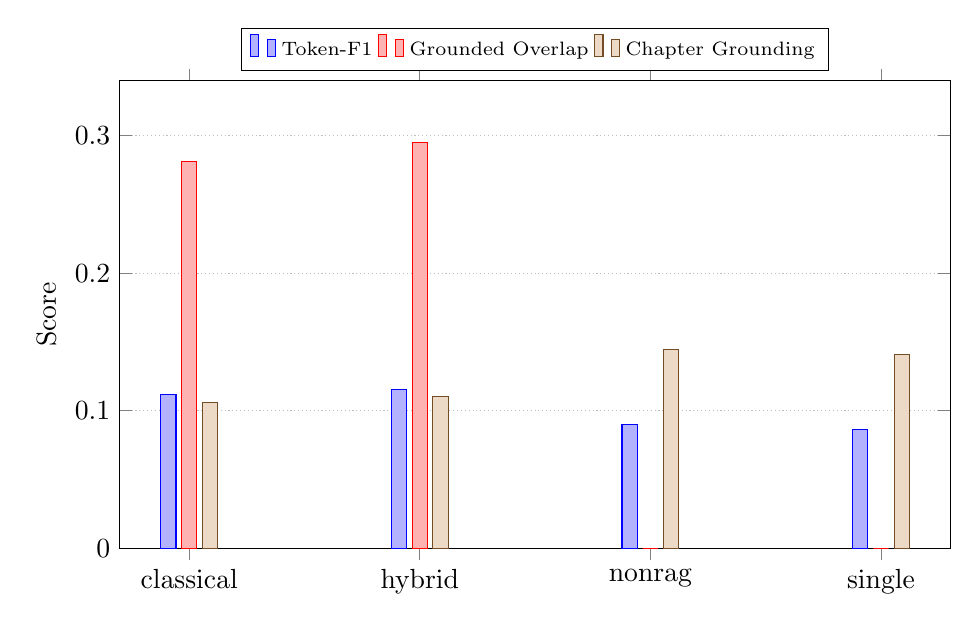
\begin{tikzpicture}
\begin{axis}[
    width=\columnwidth,
    height=0.62\columnwidth,
    ybar,
    bar width=5.5pt,
    ymin=0,
    ymax=0.34,
    symbolic x coords={classical,hybrid,nonrag,single},
    xtick=data,
    ylabel={Score},
    legend style={font=\scriptsize, at={(0.5,1.02)}, anchor=south, legend columns=3},
    ymajorgrids=true,
    grid style=densely dotted
]
\addplot coordinates {(classical,0.1115) (hybrid,0.1152) (nonrag,0.0898) (single,0.0865)};
\addplot coordinates {(classical,0.2812) (hybrid,0.2953) (nonrag,0.0000) (single,0.0000)};
\addplot coordinates {(classical,0.1057) (hybrid,0.1101) (nonrag,0.1445) (single,0.1411)};
\legend{Token-F1,Grounded Overlap,Chapter Grounding}
\end{axis}
\end{tikzpicture}
\caption{TutorEval lexical and grounding metrics. Hybrid Fast dominates token-level and retrieval-grounded overlap, while chapter grounding peaks in non-RAG settings because this metric can also fire via chapter-context overlap.}
\label{fig:tutoreval_grounding_profile}
\end{figure}

\begin{figure}[t]
\centering
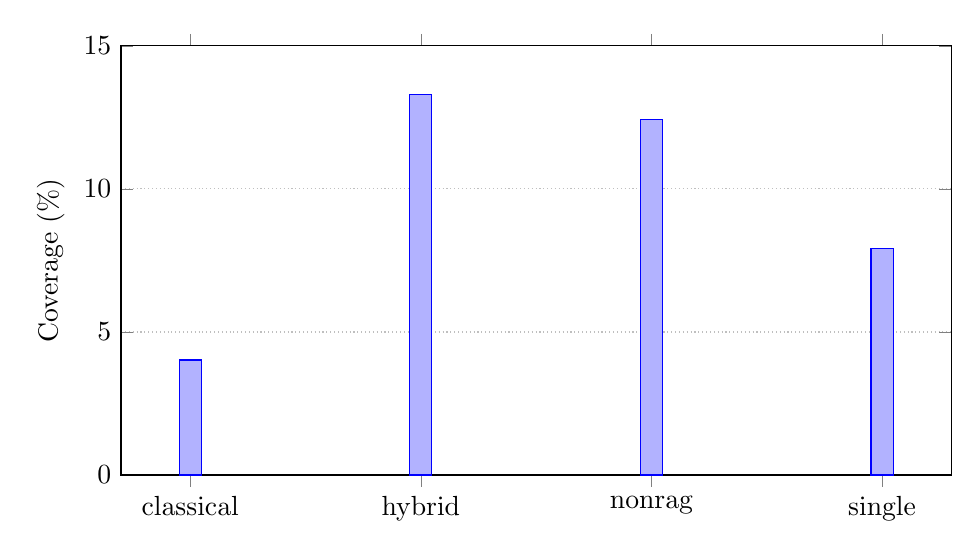
\begin{tikzpicture}
\begin{axis}[
    width=\columnwidth,
    height=0.58\columnwidth,
    ybar,
    bar width=8pt,
    ymin=0,
    ymax=15,
    symbolic x coords={classical,hybrid,nonrag,single},
    xtick=data,
    ylabel={Coverage (\%)},
    ymajorgrids=true,
    grid style=densely dotted
]
\addplot coordinates {(classical,4.02) (hybrid,13.31) (nonrag,12.42) (single,7.93)};
\end{axis}
\end{tikzpicture}
\caption{EduBench completion coverage at freeze time. Hybrid and non-RAG multi-agent are currently processing at more than $3\times$ the observed classical coverage level in this ongoing run.}
\label{fig:edubench_coverage_snapshot}
\end{figure}

\begin{figure}[t]
\centering
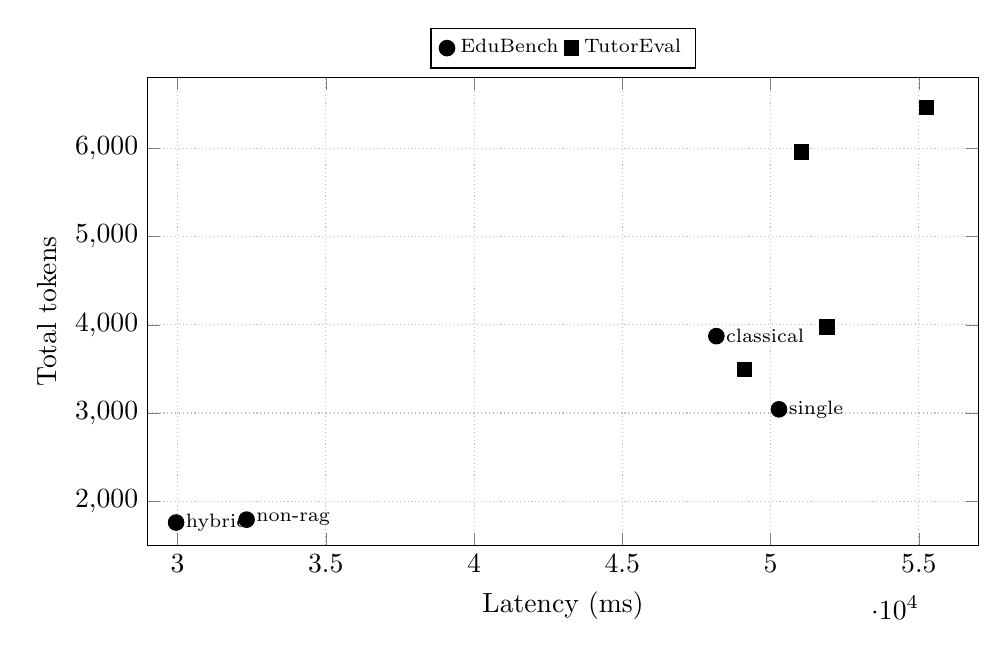
\begin{tikzpicture}
\begin{axis}[
    width=\columnwidth,
    height=0.62\columnwidth,
    xlabel={Latency (ms)},
    ylabel={Total tokens},
    legend style={font=\scriptsize, at={(0.5,1.02)}, anchor=south, legend columns=2},
    xmajorgrids=true,
    ymajorgrids=true,
    grid style=densely dotted,
    xmin=29000,
    xmax=57000,
    ymin=1500,
    ymax=6800
]
\addplot[only marks, mark=*, mark size=2.8pt] coordinates {
    (48170.2,3871.4)
    (29950.7,1757.8)
    (32327.2,1790.7)
    (50282.8,3041.5)
};
\addlegendentry{EduBench}
\addplot[only marks, mark=square*, mark size=2.6pt] coordinates {
    (51903.1,3974.7)
    (49113.4,3490.3)
    (51048.0,5959.3)
    (55257.3,6466.2)
};
\addlegendentry{TutorEval}
\node[font=\scriptsize, anchor=west] at (axis cs:29950.7,1757.8) {hybrid};
\node[font=\scriptsize, anchor=west] at (axis cs:32327.2,1790.7) {non-rag};
\node[font=\scriptsize, anchor=west] at (axis cs:48170.2,3871.4) {classical};
\node[font=\scriptsize, anchor=west] at (axis cs:50282.8,3041.5) {single};
\end{axis}
\end{tikzpicture}
\caption{Latency-token frontier on frozen summaries. Hybrid Fast remains on the most favorable region of the observed quality-efficiency surface across both datasets.}
\label{fig:latency_token_frontier}
\end{figure}

\begin{figure}[t]
\centering
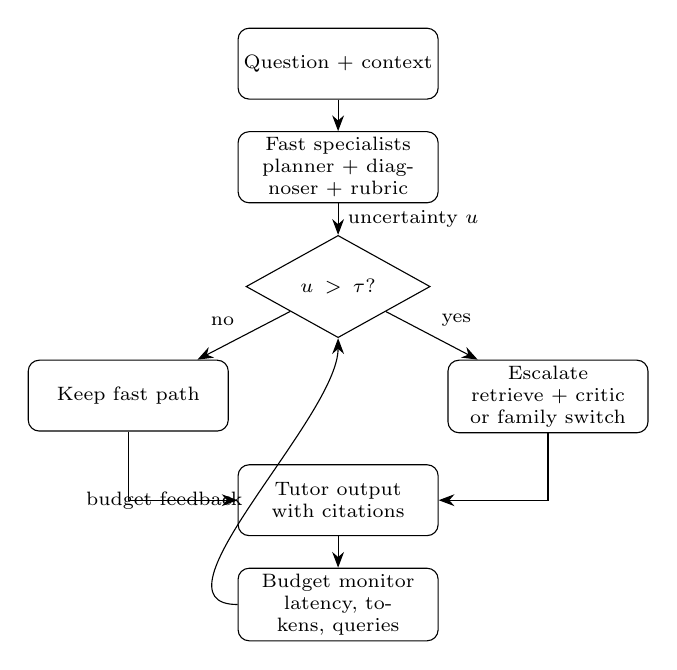
\begin{tikzpicture}[
    node distance=4mm and 6mm,
    every node/.style={font=\scriptsize, align=center},
    box/.style={draw, rounded corners, minimum height=0.9cm, text width=2.4cm, inner sep=2pt},
    decision/.style={draw, diamond, aspect=1.8, inner sep=1pt, text width=1.8cm},
    >={Stealth[length=2mm]}
]
\node[box] (in) {Question + context};
\node[box, below=of in] (fast) {Fast specialists\\planner + diagnoser + rubric};
\node[decision, below=of fast] (u) {$u > \tau$?};
\node[box, below left=6mm and 8mm of u] (keep) {Keep fast path};
\node[box, below right=6mm and 8mm of u] (esc) {Escalate\\retrieve + critic\\or family switch};
\node[box, below=16mm of u] (out) {Tutor output\\with citations};
\node[box, below=of out] (budget) {Budget monitor\\latency, tokens, queries};

\draw[->] (in) -- (fast);
\draw[->] (fast) -- node[right] {uncertainty $u$} (u);
\draw[->] (u) -- node[above left] {no} (keep);
\draw[->] (u) -- node[above right] {yes} (esc);
\draw[->] (keep) |- (out.west);
\draw[->] (esc) |- (out.east);
\draw[->] (out) -- (budget);
\draw[->] (budget.west) .. controls +(-1.2,0) and +(0,-1.0) .. node[left] {budget feedback} (u.south);
\end{tikzpicture}
\caption{Proposed CBRH-2 controller: uncertainty-aware escalation under explicit budget monitoring. The system remains in the cheap specialist path unless expected utility gain justifies additional retrieval or critique cost.}
\label{fig:cbrh2_controller}
\end{figure}


\end{document}
